%=======================================================================
%  CSE 406 — Cyber Security Sessional, Project 2026
%  TCP Reset Attack on Video Streaming — FINAL REPORT
%  Group 03, Section A1
%
%  HOW TO COMPILE:
%     pdflatex report.tex   (run twice so refs/toc resolve)
%
%  SCREENSHOTS:
%     Put your images in  report/images/  and REPLACE each
%     \ssplaceholder{...}{filename.png}  with
%     \includegraphics[width=0.9\linewidth]{filename.png}
%     The chat message accompanying this file lists exactly which
%     screenshot goes in each placeholder.
%
%  THINGS TO FILL:  every  \FILL{...}  marks a value you should edit
%     (measured numbers, IPs/MACs, OS versions, etc.).
%=======================================================================
\documentclass[11pt,a4paper]{article}

\usepackage[margin=1in]{geometry}
\usepackage{graphicx}
\usepackage{booktabs}
\usepackage{array}
\usepackage{xcolor}
\usepackage{listings}
\usepackage{enumitem}
\usepackage{caption}
\usepackage{fancyhdr}
\usepackage{tikz}
\usetikzlibrary{positioning,arrows.meta,shapes.geometric}
\usepackage[hidelinks]{hyperref}

\graphicspath{{images/}}

% --- editable-value marker (renders in orange so you can spot every TODO) ---
\newcommand{\FILL}[1]{{\color{orange!85!black}\textbf{[#1]}}}

% --- screenshot placeholder box: replace with \includegraphics when ready ---
\newcommand{\ssplaceholder}[2]{%
  \begin{center}
  \setlength{\fboxsep}{10pt}%
  \fbox{\parbox[c][4.2cm][c]{0.86\linewidth}{\centering
      \textbf{[\,Screenshot placeholder\,]}\\[6pt]
      #1\\[8pt]
      {\small Replace this box with:\ \texttt{\detokenize{#2}}}}}
  \end{center}}

% --- terminal / code listing style ---
\definecolor{codebg}{gray}{0.96}
\lstdefinestyle{term}{
  basicstyle=\ttfamily\footnotesize,
  backgroundcolor=\color{codebg},
  breaklines=true, columns=fullflexible,
  frame=single, framerule=0pt, xleftmargin=6pt, xrightmargin=6pt,
  keepspaces=true, showstringspaces=false, aboveskip=6pt, belowskip=6pt,
}
\lstset{style=term}
\newcommand{\code}[1]{\texttt{\detokenize{#1}}}

\pagestyle{fancy}\fancyhf{}
\rhead{\small TCP Reset Attack on Video Streaming}
\lhead{\small CSE 406 — Group 03}
\cfoot{\thepage}
\renewcommand{\headrulewidth}{0.4pt}

\captionsetup{font=small,labelfont=bf}

%=======================================================================
\begin{document}

%------------------------- Title block --------------------------------
\begin{center}
  {\large\scshape Bangladesh University of Engineering and Technology}\\[2pt]
  {\small Department of Computer Science and Engineering}\\[10pt]
  {\small CSE 406 — Cyber Security Sessional \quad|\quad Project 2026: Attack Tools Implementation}\\[16pt]
  \rule{\linewidth}{0.6pt}\\[6pt]
  {\LARGE\bfseries TCP Reset Attack on Video Streaming}\\[4pt]
  {\large Final Project Report}\\[4pt]
  \rule{\linewidth}{0.6pt}\\[12pt]

  \begin{tabular}{ll}
    \textbf{Group:} & 03, Section A1\\[4pt]
    \textbf{Members:} & 2105004 — Fahim Ishtiak\\
                      & 2105001 — Nahid Hossain Redom\\[4pt]
    \textbf{Date:} & September 19, 2026\\
  \end{tabular}
\end{center}
\vspace{6pt}
\hrule
\vspace{10pt}

%------------------------- Abstract -----------------------------------
\begin{abstract}
\noindent
This report documents the implementation and evaluation of a \textbf{TCP Reset
(RST) injection attack} against an active video-streaming session, together with
the defenses that stop it. TCP does not authenticate its control segments, so an
attacker who knows a connection's four-tuple and a valid sequence number can
forge an RST and tear the connection down. Because both switched LANs and Wi-Fi
deliver unicast frames only to their intended recipient, our attacker first uses
\textbf{ARP cache poisoning} to become a man-in-the-middle (MITM), reads the live
sequence numbers off the relayed stream, and injects a forged RST that stalls
playback. We report the attack process, the expected versus the actual outcome
(and the reasons they differ), the defense mechanisms and whether they behaved as
expected, and the assumptions underlying the whole demonstration. The attack and
both defense layers were demonstrated successfully on \textbf{three separate
physical machines} over a controlled Wi-Fi LAN.
\end{abstract}

\tableofcontents
\vspace{8pt}\hrule

%=======================================================================
\section{Introduction and Objective}
A TCP connection is identified only by its four-tuple (source IP, source port,
destination IP, destination port) plus a 32-bit sequence-number space; it has no
cryptographic authentication of control-plane segments. If an attacker sends a
spoofed segment with the RST flag, the correct four-tuple, and a sequence number
the receiver's stack accepts, the receiver tears the connection down as if the
peer had hung up.

Video streaming is an instructive target because a single long-lived TCP
connection carries the whole session: it gives an on-path attacker a wide
observability window, and a full reset produces a visible, measurable failure
(playback stalls, the player reports a connection error, and the socket vanishes
from both peers' connection tables) rather than the momentary glitch a single
dropped packet would cause.

\medskip\noindent\textbf{Objective.} Build the tooling to (i) become on-path via
ARP poisoning, (ii) sniff the live sequence numbers, and (iii) inject a forged
RST that terminates a streaming connection; then demonstrate and evaluate the
defenses that prevent it.

%=======================================================================
\section{Threat Model, Environment, and Assumptions}
\label{sec:assumptions}

\subsection{Threat model}
We scope the project to an \textbf{on-path (LAN-local) attacker}: a host on the
same broadcast domain as the victims that makes itself on-path via ARP poisoning,
so it can \emph{read} the exact live sequence number rather than guessing it
blindly. A true off-path (blind) attacker would additionally have to defeat
source-port randomization and brute-force a valid sequence number — a much harder
attack that RFC~5961 (Section~\ref{sec:defense}) makes impractical.

\subsection{Demonstration environment}
The demonstration used three physical machines on one Wi-Fi access point that we
control (AP/client isolation disabled). No third-party, campus, or production
traffic was ever touched.

\begin{table}[h]\centering
\begin{tabular}{@{}llll@{}}
\toprule
\textbf{Machine} & \textbf{Role} & \textbf{OS} & \textbf{Address}\\
\midrule
PC~1 & Video server (victim) & Windows/Ubuntu & IP 10.169.169.216, MAC 98:59:7a:cb:16:8c\\
PC~2 & Client / player (victim) & Windows & IP 10.169.169.114, MAC 90:e8:68:4a:a3:a5\\
PC~3 & Attacker & Linux mint & IP 10.169.169.133, MAC dc:21:5c:82:1e:8c\\
\midrule
\multicolumn{4}{@{}l}{Link layer: Wi-Fi access point - Mobile Hotspot, subnet 10.169.169.0/24}\\
\bottomrule
\end{tabular}
\caption{Physical test-bed for the demonstration. One victim was Windows and one
was Linux; the attacker must be Linux (raw sockets, Scapy, IP forwarding).}
\label{tab:env}
\end{table}

\subsection{Assumptions}
The demonstration relies on the following assumptions; each is a real
precondition of the attack, and each maps to a defense in
Section~\ref{sec:defense}.
\begin{enumerate}[leftmargin=1.4em,itemsep=2pt]
  \item \textbf{Shared Layer-2 segment.} All three hosts are in one broadcast
        domain so the attacker's forged ARP replies reach the victims. On Wi-Fi
        this means \textbf{AP/client isolation is OFF}; with it on, the attacker
        cannot even reach the victims and poisoning never lands.
  \item \textbf{On-path via ARP, not passive sniffing.} A switch/AP forwards
        unicast only to the destination MAC, so passive promiscuous sniffing
        alone does \emph{not} reveal the server$\leftrightarrow$client flow; ARP
        poisoning is what provides visibility.
  \item \textbf{Clean MITM (IP forwarding on).} The attacker enables IP
        forwarding so the relayed stream keeps flowing; otherwise it is a
        black-hole DoS, not the RST attack under study.
  \item \textbf{Single long-lived TCP connection.} We use a custom raw-TCP
        streamer so the whole session is one connection that a single RST tears
        down (we deliberately avoid QUIC/HTTP-3, which has no RST, and
        many-short-connection HLS/DASH, which masks a single reset).
  \item \textbf{Attacker is Linux.} ARP spoofing and raw RST injection need raw
        sockets, Scapy, and \code{/proc/sys/net/ipv4/ip_forward}.
  \item \textbf{Modern victim kernels implement RFC~5961} (exact-match RST
        rule) — this is what makes the on-path position \emph{necessary} and is
        the baseline TCP defense we evaluate.
  \item \textbf{No ARP hardening by default.} Victims start with dynamic ARP; the
        defense (Section~\ref{sec:defense}) removes this assumption on purpose.
  \item \textbf{Real MAC known before pinning.} The static-ARP defense assumes we
        can learn each peer's genuine MAC before the attacker starts (or read it
        on the peer directly).
\end{enumerate}

%=======================================================================
\section{Attack Process}
\label{sec:attack}

The attack has two stages: get on-path (ARP poisoning), then read-and-inject
(sniff sequence numbers, forge the RST). Figure~\ref{fig:topo} shows the
topology; Section~\ref{sec:attack-steps} walks through the timeline.

\subsection{Topology}
\begin{figure}[h]\centering
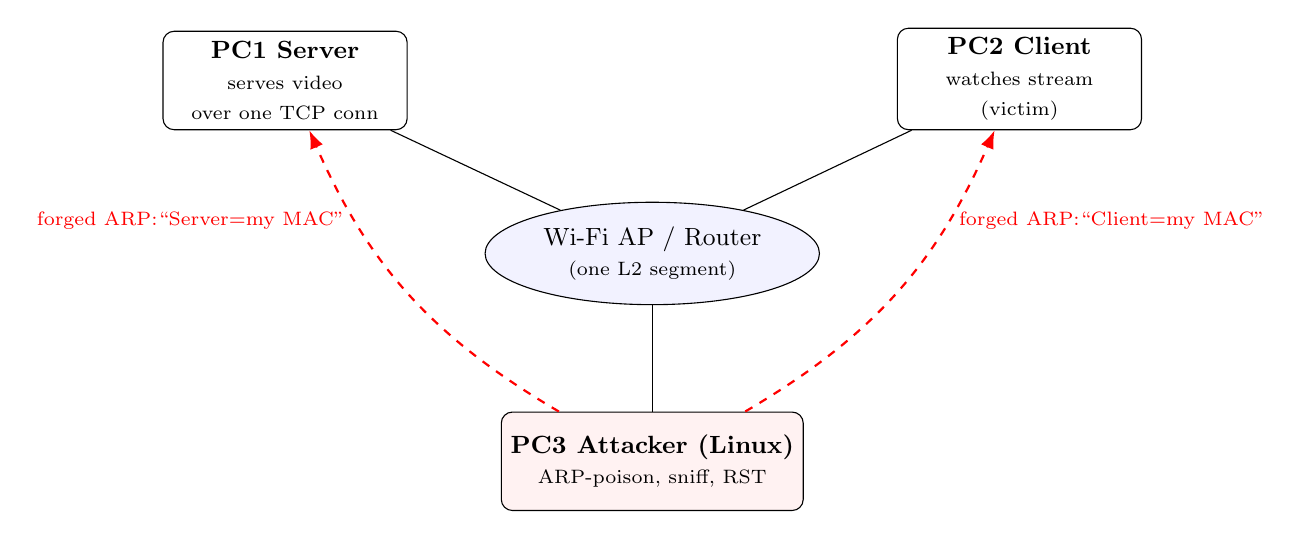
\begin{tikzpicture}[
    box/.style={draw,rounded corners,align=center,minimum width=3.1cm,minimum height=1.25cm,font=\small},
    ap/.style={draw,ellipse,align=center,minimum width=3.2cm,minimum height=1.3cm,font=\small,fill=blue!5},
    >=Latex]
  \node[ap] (ap) {Wi-Fi AP / Router\\\scriptsize (one L2 segment)};
  \node[box,above left=1.1cm and 1.6cm of ap] (srv) {\textbf{PC1 Server}\\\scriptsize serves video\\\scriptsize over one TCP conn};
  \node[box,above right=1.1cm and 1.6cm of ap] (cli) {\textbf{PC2 Client}\\\scriptsize watches stream\\\scriptsize (victim)};
  \node[box,below=1.35cm of ap,fill=red!5] (att) {\textbf{PC3 Attacker (Linux)}\\\scriptsize ARP-poison, sniff, RST};
  \draw (srv) -- (ap); \draw (cli) -- (ap); \draw (att) -- (ap);
  \draw[->,red,dashed,thick] (att) to[bend left=18] node[near end,left,font=\scriptsize,red]{forged ARP:\\ ``Server=my MAC''} (srv);
  \draw[->,red,dashed,thick] (att) to[bend right=18] node[near end,right,font=\scriptsize,red]{forged ARP:\\ ``Client=my MAC''} (cli);
\end{tikzpicture}
\caption{Phase-2 physical topology. On a switched/Wi-Fi LAN the attacker cannot
passively see the server$\leftrightarrow$client unicast flow; it poisons both
victims' ARP caches so the traffic transits it (a clean MITM with IP forwarding
on), then injects the forged RST.}
\label{fig:topo}
\end{figure}

\subsection{Stage 1 — ARP cache poisoning (becoming MITM)}
The attacker (\code{attacker/arp_spoof.py}) resolves the real MACs of the server
and client, enables IP forwarding, then repeatedly sends forged ARP
\emph{replies}: to the client, ``\emph{server IP} is at \emph{attacker MAC}''; to
the server, ``\emph{client IP} is at \emph{attacker MAC}''. Both victims update
their caches and send their traffic to the attacker, which relays it onward. The
stream keeps playing — a \emph{clean MITM}, not a DoS — but every segment now
passes through the attacker, who can read it. On stop, the tool restores the real
bindings.

\subsection{Stage 2 — Sniff live sequence numbers and inject the RST}
\label{sec:attack-steps}
The injector (\code{attacker/rst_attack.py}) runs two threads:
\begin{itemize}[leftmargin=1.4em,itemsep=2pt]
  \item \textbf{Sniffer} — learns the connection's live state from the relayed
        traffic: the client's \code{RCV.NXT} is read directly from the ack field
        of the client's own ACKs (authoritative), along with the server's data
        frontier. It ignores RST/SYN packets so it never learns from its own
        injected RSTs.
  \item \textbf{Sender} — hammers forged RSTs at both endpoints: to the client
        spoofing the server as source, and (by default) to the server spoofing
        the client. Each shot is a small \textbf{burst stepped by $\pm$1~MSS}
        around the learned \code{RCV.NXT}.
\end{itemize}

\paragraph{Why hammer and burst (the RFC 5961 timing caveat).}
Modern Linux (RFC~5961) accepts a RST immediately only if \code{seq == RCV.NXT}
\emph{exactly}; an in-window but non-exact RST draws a harmless ``challenge ACK''.
On a fast stream \code{RCV.NXT} keeps advancing, so a single guess is usually
stale on arrival. Sustained hammering lands a shot during one of the streamer's
pacing gaps when \code{RCV.NXT} is momentarily frozen; the $\pm$MSS burst absorbs
residual drift. Resetting the \emph{server} first freezes the stream, which makes
the client-side exact match trivial. Notably, the Scapy/Python implementation
with this burst strategy was fast enough — the C/raw-socket hot path mentioned as
a contingency in the proposal was \emph{not} required.

\paragraph{One-command driver.} \code{phase2/attacker/run_attack.sh} auto-detects
the LAN interface, starts poisoning, waits for the MITM to settle, then launches
the injector; Ctrl+C stops it and restores ARP (see
Section~\ref{sec:obs-impl} for a robustness fix made here).

\begin{figure}[h]\centering
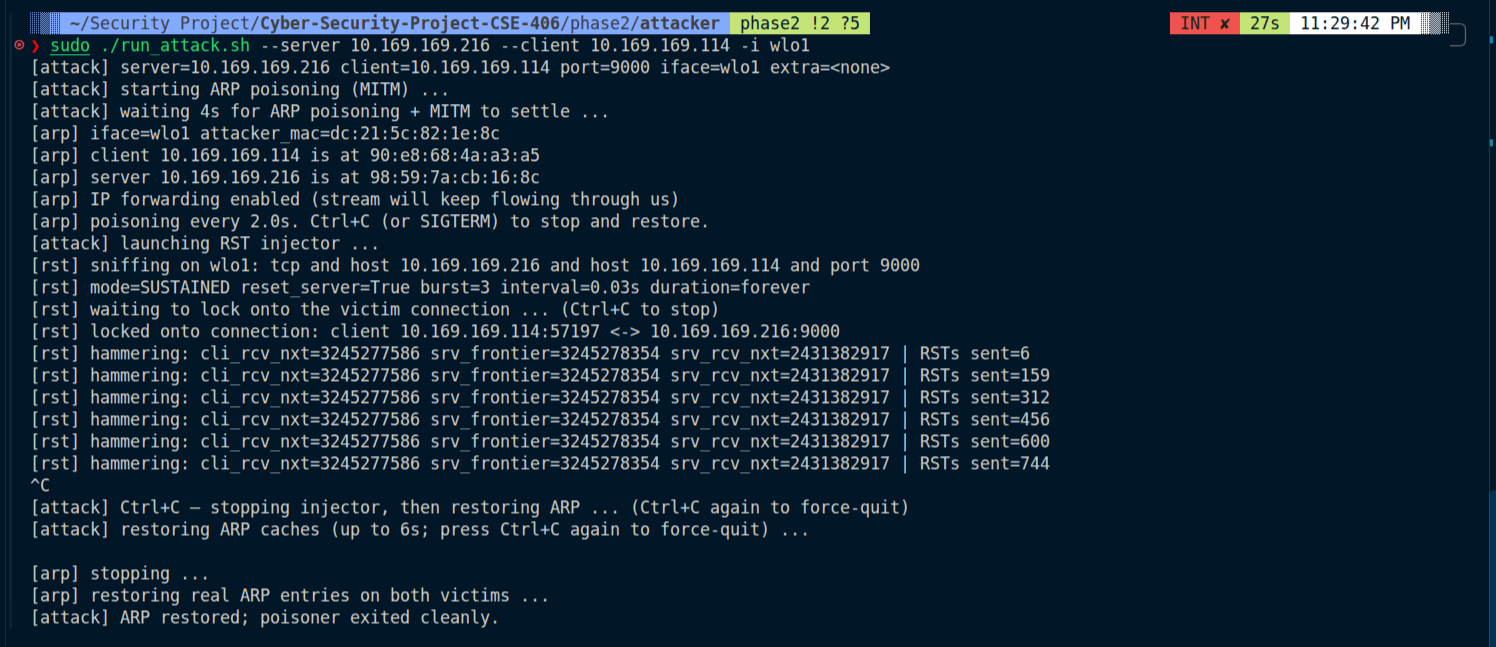
\includegraphics[width=0.95\linewidth]{fig_attacker_rst.png}
\caption{Attacker driver (\code{run_attack.sh}). It resolves the victims' real
MACs, enables IP forwarding, poisons both caches, then locks onto
\code{10.169.169.114:57197 <-> 10.169.169.216:9000} and hammers forged RSTs. The
tracked \code{cli_rcv_nxt}/\code{srv_frontier} are already \emph{frozen} at the
first report (\code{RSTs sent=6}) — the stream reset almost immediately — after
which sustained mode keeps hammering (to \code{RSTs sent=744}) until Ctrl+C
cleanly restores ARP.}
\label{fig:attacker}
\end{figure}

%=======================================================================
\section{Expected Outcome}
\label{sec:expected}
From the design proposal (Section~5), a successful attack should produce:
\begin{itemize}[leftmargin=1.4em,itemsep=2pt]
  \item \textbf{On the wire:} a Wireshark capture showing the injected RST
        immediately after a run of normal data segments, with \emph{no preceding
        FIN/FIN-ACK} — visually distinct from a graceful close.
  \item \textbf{At the client:} the stream's entry disappears from the connection
        table (\code{ss}/\code{netstat}); the player stalls once its buffer
        drains and reports a network/connection error.
  \item \textbf{At the server (if targeted):} the corresponding half of the
        connection is torn down and the streaming socket terminates.
  \item \textbf{Measurable:} a success rate over repeated trials, a
        time-to-disruption, and the number of RST attempts per success (a proxy
        for the RFC~5961 timing drift).
\end{itemize}

%=======================================================================
\section{Actual Outcome}
\label{sec:actual}
On the three-machine Wi-Fi test-bed the attack behaved as predicted.

\begin{itemize}[leftmargin=1.4em,itemsep=2pt]
  \item \textbf{Clean MITM confirmed.} The attacker resolved both victims' real
        MACs and enabled IP forwarding (Figure~\ref{fig:attacker}); the stream
        then played normally while transiting the attacker — playback started
        after the 3\,s prebuffer and advanced with a healthy buffer
        (Figure~\ref{fig:mitm}) — a clean MITM, not a DoS.
  \item \textbf{Teardown observed.} The client printed the RST banner (``reset
        with NO preceding FIN''), the download froze at \code{30.4\%}
        (\code{1.74/5.70 MB}), and it reported \textbf{PLAYBACK STALLED}
        (Figure~\ref{fig:stall}).
  \item \textbf{Connection table cleared.} On the Windows victim,
        \code{netstat -ano | findstr :9000} listed the four-tuple on port~9000
        \emph{while} streaming and showed \textbf{nothing after the reset} ---
        confirming (per proposal~\S5) that the socket was destroyed, not merely
        idle.
  \item \textbf{On the wire.} The attacker-side capture showed the injected
        \textbf{RST flood in both directions with no FIN} anywhere
        (Figure~\ref{fig:wireshark}).
\end{itemize}

\begin{figure}[h]\centering
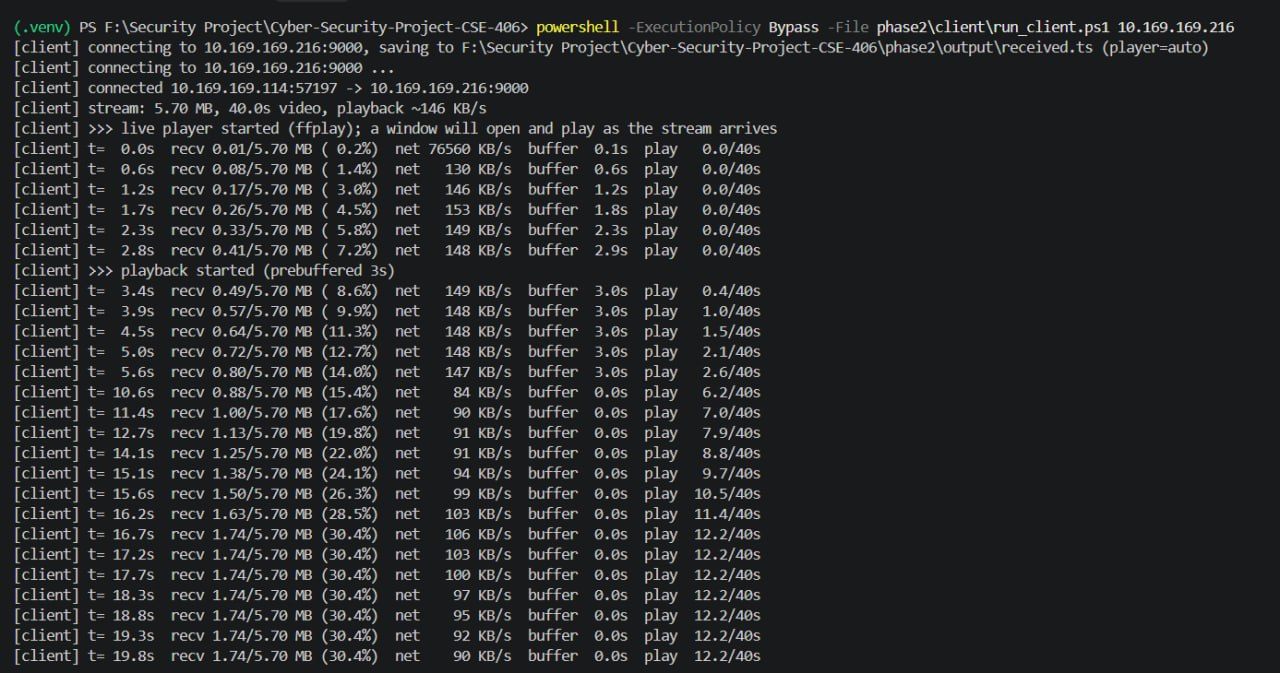
\includegraphics[width=0.95\linewidth]{fig_mitm_healthy.jpg}
\caption{Victim client during the attack (Windows, \code{run_client.ps1}). While
relayed through the attacker the stream plays normally — playback starts after the
3\,s prebuffer and advances with a healthy buffer (a \emph{clean} MITM, not a
DoS) — until the download halts at \code{1.74/5.70 MB (30.4\%)} around
\code{t=16.7s} as the injected RST freezes the server; playback then coasts on the
drained buffer until it stalls (Figure~\ref{fig:stall}).}
\label{fig:mitm}
\end{figure}

\begin{figure}[h]\centering
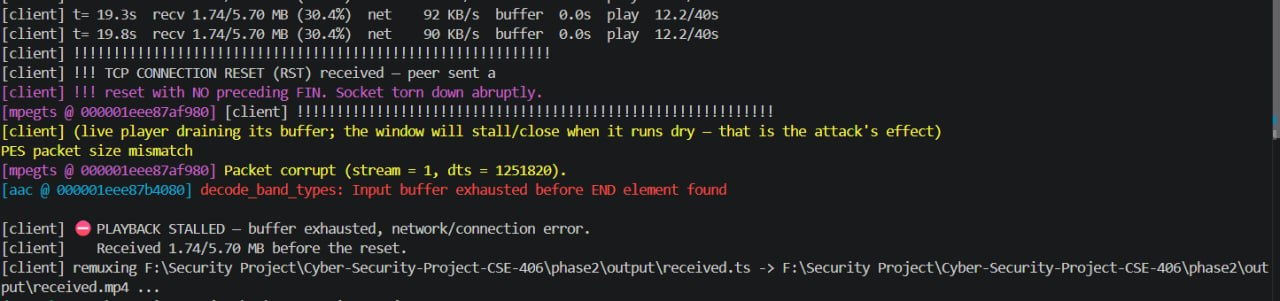
\includegraphics[width=0.95\linewidth]{fig_client_stall.jpg}
\caption{The victim experiencing the outage. The client reports ``TCP CONNECTION
RESET (RST) received --- \dots reset with NO preceding FIN'', the ffmpeg player
throws corrupt-packet / buffer-exhausted errors, and it prints \textbf{PLAYBACK
STALLED} having received only \code{1.74/5.70 MB} before the reset --- an abrupt,
FIN-less teardown, exactly the attack's intended effect.}
\label{fig:stall}
\end{figure}

% (Optional) A before/after netstat/ss screenshot could go here, but the
% connection-table teardown is reported in prose above (§6) since it was observed
% live on the Windows victim. To add it, drop an image in images/ and uncomment:
% \begin{figure}[h]\centering
%   \includegraphics[width=0.9\linewidth]{fig_ss_gone.png}
%   \caption{Client connection table before vs.\ after: the ESTABLISHED entry vanishes.}
%   \label{fig:ss}
% \end{figure}

\begin{figure}[h]\centering
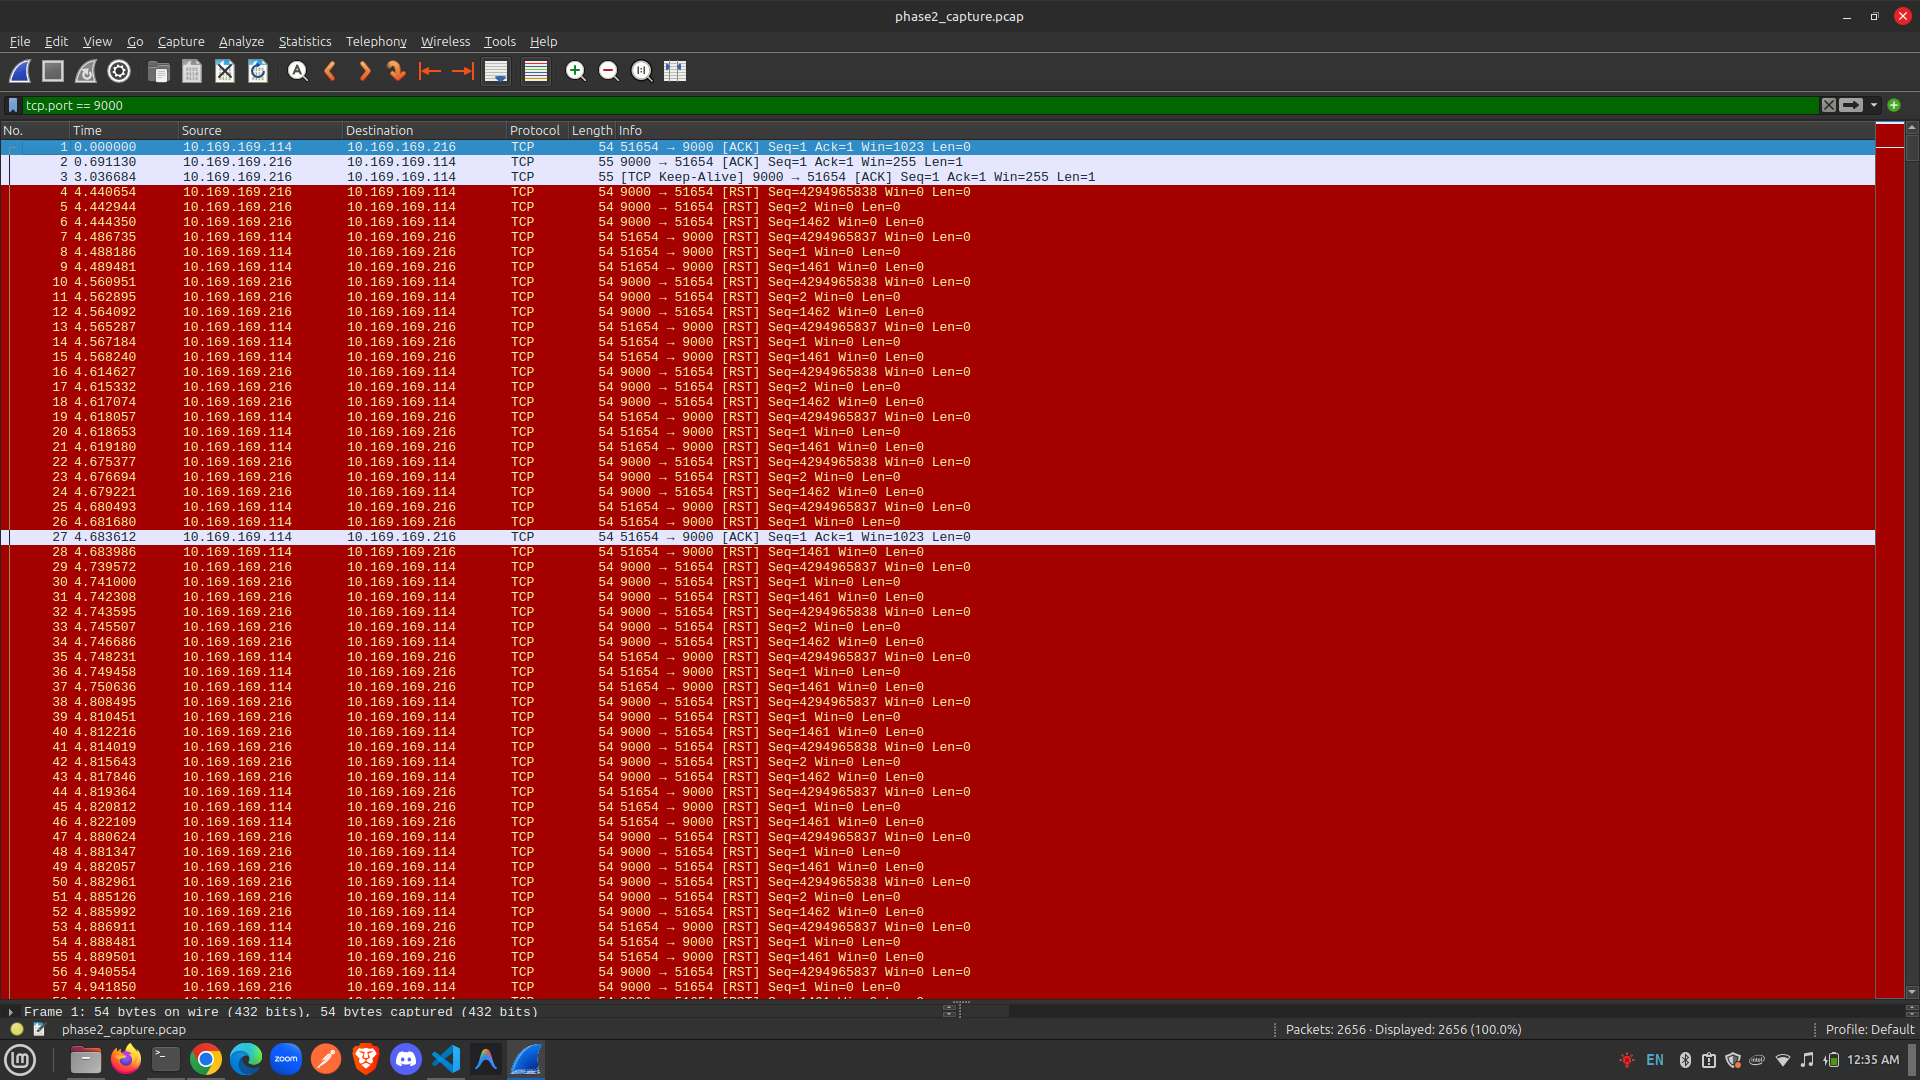
\includegraphics[width=0.97\linewidth]{fig_wireshark_rst.png}
\caption{Attacker-side capture (filter \code{tcp.port == 9000}). A sustained flood
of forged \textbf{RST} segments in \emph{both} directions: \code{9000\,$\to$\,51654}
carries the \textbf{server's} IP (\code{10.169.169.216}) as source, and
\code{51654\,$\to$\,9000} carries the \textbf{client's} IP — yet both were sent by
the attacker. The sequence values (\code{Seq=1/1461/1462}, and \code{4294965838}
= $-1$~MSS relative) are the $\pm$1~MSS burst around \code{RCV.NXT}, all
\code{Win=0}, \code{Len=0}. Crucially there is \textbf{no FIN/FIN-ACK} anywhere —
the RFC~5961 exact-match burst strategy tearing the connection down abruptly.}
\label{fig:wireshark}
\end{figure}

\subsection{Measured results}
\begin{table}[h]\centering
\begin{tabular}{@{}p{3.5cm}p{4.4cm}p{6.3cm}@{}}
\toprule
\textbf{Metric} & \textbf{How measured} & \textbf{Result}\\
\midrule
Attack success rate & successful resets over repeated trials & 100\% --- succeeded on every attempt\\[2pt]
Time-to-disruption & injector lock-on $\to$ stream frozen & $<1$\,s: the tracked sequence values were already static at the first report; the client's playback stalled within a few seconds\\[2pt]
RST attempts per success & injector \code{RSTs sent=} counter at teardown & Reset landed by the first report (\code{RSTs sent=6}); sustained mode then continued to \code{744} by design\\[2pt]
Behavior vs.\ client retry & default client vs.\ \code{RECONNECT=1} & Default client stalled and stopped (no retry); sustained hammering is what keeps a reconnecting client down\\[2pt]
Success with vs.\ without defense & rerun with static ARP pinned on both victims & Without defense: reset every time. With defense: attack fails (\S\ref{sec:defense})\\
\bottomrule
\end{tabular}
\caption{Measured results on the three-machine Wi-Fi test-bed (design proposal
Table~2). The attack succeeded on every run; exact per-run RST counts were not
tallied, but the injector's live counter and the frozen sniffer state
(Figure~\ref{fig:attacker}) show the reset landing near-instantly.}
\label{tab:metrics}
\end{table}

%=======================================================================
\section{Differences from the Plan, and Why}
\label{sec:diff}
The \emph{logical} attack matched the proposal exactly; the differences are in
deployment and implementation, and all are documented here rather than hidden.

\begin{enumerate}[leftmargin=1.4em,itemsep=4pt]
  \item \textbf{Docker Phase~1 was built but is not reported here; the results
        come from three physical machines.} The proposal planned a single-host
        Docker simulation (Phase~1) before the physical demo (Phase~2). We did
        build and run the Docker-based setup, but could not get it working across
        three separate machines, so we conducted the \emph{entire} reported attack
        and defense on three real machines without Docker. \emph{Impact:} none on
        the findings --- the physical demonstration is the stronger evidence,
        since it proves the attack is not an artifact of the Docker virtual
        network stack, which was the whole purpose of Phase~2.
  \item \textbf{The attacker ran natively on a physical Linux host, not in a
        VM/container.} Because there was no Docker/VM layer, the Wi-Fi + VM
        ``bridged networking'' pitfalls anticipated for a virtualized attacker
        did not arise: a native Linux station is a genuine Layer-2 peer, so ARP
        poisoning worked directly.
  \item \textbf{Scapy/Python was sufficient; no C hot path.} The proposal held a
        C/raw-socket reimplementation in reserve in case injection latency was
        too high. The sniff-and-hammer loop with the $\pm$MSS burst around
        \code{RCV.NXT} (and resetting the server first to freeze the stream) made
        the exact-match land reliably, so the C path was unnecessary.
  \item \textbf{Mixed-OS victims required a cross-platform defense.} With one
        Windows and one Linux victim, the single Linux/Docker helper from the
        proposal was expanded into a cross-platform defense suite
        (Section~\ref{sec:defense}).
  \item \textbf{An implementation robustness fix} was made to the attacker's
        shutdown path (Section~\ref{sec:obs-impl}); it does not change the attack
        result but was necessary for clean, repeatable demos.
\end{enumerate}

%=======================================================================
\section{Defense Mechanisms and Evaluation}
\label{sec:defense}
Following the proposal (Section~6), the defense has two complementary layers.

\subsection{Primary (TCP layer): RFC 5961 strict sequence validation}
Modern Linux implements RFC~5961: an RST is accepted only if
\code{seq == RCV.NXT} exactly; an in-window non-exact RST yields a challenge ACK.
This narrows a blind attacker's valid guess space from the whole window to a
single value, so it \emph{defeats an off-path attacker}. It does \emph{not} stop
our on-path attacker, who reads the exact value off the wire — which is precisely
why the ARP-layer defense is also needed. We verify the kernel behavior with
\code{phase2/defense/rfc5961_check.sh}.

\subsection{Complementary (ARP layer): stop the MITM from forming}
Since the attack depends on ARP poisoning, preventing it removes the on-path
position entirely. We implemented the host-side defenses (the managed-switch
equivalent, Dynamic ARP Inspection, was unavailable on our consumer AP):

\begin{itemize}[leftmargin=1.4em,itemsep=2pt]
  \item \textbf{Static ARP entries (prevention).} Pin each peer's real IP$\to$MAC
        as a permanent entry so forged ARP replies are ignored.
        Cross-platform: \code{static_arp.sh} (Linux/macOS) and
        \code{static_arp.ps1} (Windows).
  \item \textbf{ARP monitoring (detection).} \code{arp_watch.py} runs on a victim
        and raises an alert on an ARP-poisoning attempt. On Linux (\code{--sniff})
        it reads ARP frames directly off the wire, so it flags the forged reply
        \emph{even while the static pin silently blocks it} (a pinned host's ARP
        table never changes, so table polling alone would see nothing); without
        \code{--sniff} it polls the neighbour table for a changed binding. It can
        optionally re-pin automatically. This is the host-side stand-in for DAI.
  \item \textbf{One-command driver.} \code{defend.sh}/\code{defend.ps1} pins the
        peer (and gateway) and starts the monitor; a \code{--off}/\code{-Off}
        switch removes the entries again, so the defense can be toggled
        \emph{on and off} to show the attack first, then the defense.
\end{itemize}

\paragraph{The defense runs on BOTH victims.} To read the sequence numbers the
attacker must see the traffic, which needs \emph{both} caches poisoned. Pinning
only the client leaves the server poisoned (so the attacker still sees the
server$\to$client half and can still forge RSTs) — partial protection. Pinning
\textbf{both} means neither direction transits the attacker, it sees nothing, and
the attack collapses to the blind case RFC~5961 already defeats — full
protection.

\subsection{Does the defense work as expected?}
\textbf{Yes.} With static ARP pinned on both victims and the attack re-run:
\begin{itemize}[leftmargin=1.4em,itemsep=2pt]
  \item the client \textbf{kept playing} — no RST banner, status lines kept
        advancing (Figure~\ref{fig:defense-ok});
  \item the attacker's injector \textbf{never locked on} — it stayed at
        ``waiting to lock onto the victim connection\dots'' because poisoning no
        longer redirected the flow;
  \item \code{arp_watch.py} printed an \textbf{ARP POISONING} alert for each
        forged reply — visible proof the attempt happened and was neutralised
        (Figure~\ref{fig:defense-ok}); the pinned entry did not move
        (\code{verify} $\to$ \code{OK}).
\end{itemize}
This confirms the proposal's claim that the ARP and TCP defenses are
complementary: RFC~5961 stops the blind case, and static ARP/monitoring removes
the on-path position that defeats RFC~5961.

\begin{figure}[h]
\ssplaceholder{Split view with the defense ON: (left) client still streaming
normally during the attack; (right) \code{arp_watch.py} printing ``ARP
POISONING\dots'' alerts and/or \code{static_arp verify} showing OK. Optionally
include \code{rfc5961_check.sh} output.}{images/fig_defense.png}
\caption{Defense working: with both victims pinned, the MITM never forms — the
client keeps playing while the monitor flags every neutralised poisoning attempt.}
\label{fig:defense-ok}
\end{figure}

%=======================================================================
\section{Observations}
\label{sec:obs}

\subsection{On the attack}
\begin{itemize}[leftmargin=1.4em,itemsep=2pt]
  \item Passive sniffing alone revealed \emph{nothing} of the video flow on the
        Wi-Fi LAN — the ARP-poisoning MITM was genuinely necessary, confirming
        the ``learning switch / AP'' premise.
  \item The MITM was ``clean'': playback continued unaffected while relayed,
        which is what makes the later reset a convincing, isolated event.
  \item Resetting the server first (freezing \code{RCV.NXT}) made the client-side
        exact match land quickly; \code{--no-server} (client only) took more
        attempts, directly illustrating the RFC~5961 drift effect.
  \item With \code{RECONNECT=1} the client re-opened a new connection after a
        reset, so \textbf{sustained} injection was needed to keep it down — the
        auto-retry behavior the proposal said to measure, not hide.
\end{itemize}

\subsection{On the implementation (robustness fix)}
\label{sec:obs-impl}
During repeated runs we found that stopping \code{run_attack.sh} with Ctrl+C could
hang while ``restoring ARP''. Root cause: a shell background job
(\code{arp_spoof.py} started with \code{\&}) has \textbf{SIGINT set to ignored}
(POSIX behavior when job control is off), so the cleanup's \code{kill -INT} was a
no-op and the parent's \code{wait} blocked forever. We fixed this by (i) having
\code{arp_spoof.py} install explicit SIGINT/SIGTERM handlers and always complete
its ARP restore, and (ii) rewriting the driver's shutdown with a counted-Ctrl+C
trap and bounded waits: \textbf{one Ctrl+C} stops and restores gracefully,
\textbf{two} force-quit immediately. This did not change the attack itself but was
essential for clean, repeatable demonstrations.

\subsection{On the defense}
\begin{itemize}[leftmargin=1.4em,itemsep=2pt]
  \item The static-ARP defense is decisive but assumes the \emph{real} MAC is
        learned before the attacker starts; pinning while already poisoned would
        pin the attacker's MAC. Reading the MAC on the peer itself avoids this.
  \item Static ARP is ``impractical at scale'' (per the proposal); \code{arp_watch}
        provides the detection role that DAI would give on a managed switch.
\end{itemize}

%=======================================================================
\section{Conclusion}
We implemented a complete, on-path TCP reset attack against a single-connection
video stream and demonstrated it end-to-end on three physical machines over
Wi-Fi: ARP poisoning to become MITM, live sequence-number sniffing, and a
burst-hammered forged RST that reliably tore the connection down and stalled
playback — matching the proposal's expected outcome. We then showed the
two-layer defense: RFC~5961 (which defeats the blind attacker but not the on-path
one) and an ARP-layer defense (static pinning plus monitoring) that removes the
on-path position and collapses the attack to the defeated blind case. The main
deviations from the plan — skipping the Docker phase in favour of the physical
demo, a native Linux attacker, an all-Scapy injector, and a cross-platform
defense for mixed-OS victims — did not weaken the result; the physical
demonstration is the stronger evidence that the attack and its defenses behave as
designed on real networks.

%=======================================================================
\appendix
\section{Reproduction commands}
\label{app:repro}
\textbf{Server (PC1)} — \code{phase2/server/run_server.sh} (Linux/macOS) or
\code{run_server.ps1} (Windows); prints its LAN IP.\\
\textbf{Client (PC2)} — \code{phase2/client/run_client.sh <SERVER_IP>} or
\code{run_client.ps1 <SERVER_IP>}.\\
\textbf{Attacker (PC3, Linux)}:
\begin{lstlisting}
cd phase2/attacker
./setup.sh
sudo ./preflight.sh --server <SERVER_IP> --client <CLIENT_IP>
sudo ./run_attack.sh --server <SERVER_IP> --client <CLIENT_IP>
# capture (optional, separate shell):
sudo ./capture.sh --server <SERVER_IP> --client <CLIENT_IP> -o ../output/phase2_capture.pcap
\end{lstlisting}
\textbf{Defense (on BOTH victims, before attacking)}:
\begin{lstlisting}
# Linux/macOS victim (pin the OTHER endpoint):
sudo phase2/defense/defend.sh --peer <PEER_IP> --peer-mac <PEER_MAC> \
     --gateway auto --watch
# Windows victim (Admin PowerShell):
phase2\defense\defend.ps1 -Peer <PEER_IP> -PeerMac <PEER_MAC> -Gateway auto -Watch
# turn the defense OFF again to re-show the attack:
sudo phase2/defense/defend.sh --peer <PEER_IP> --gateway auto --off
\end{lstlisting}

\end{document}
